\documentclass{beamer}
\usetheme{Boadilla}
\usecolortheme{sidebartab}
\beamertemplatenavigationsymbolsempty
\setbeamertemplate{footline}[frame number]
\usepackage{hyperref} 
\usepackage{graphicx}
\usepackage{color}
\usepackage{booktabs}
\usepackage{listings}
\usepackage{soul}
\usepackage{tikz}
\usepackage[utf8]{inputenc}
\usepackage{CJKutf8}
\usetikzlibrary{shapes.geometric}

\definecolor{gray}{rgb}{0.4,0.4,0.4}
\definecolor{darkblue}{rgb}{0.0,0.0,0.6}
\definecolor{cyan}{rgb}{0.0,0.6,0.6}

\lstset{
	basicstyle=\ttfamily,
	columns=fullflexible,
	showstringspaces=false,
	commentstyle=\color{gray}\upshape
}

\tikzset{node style/.style={
		draw=blue,
		thick,
		fill=blue!70,
		text=white,
		ellipse,
		minimum width=2cm,
		minimum height=0.75cm,
		font=\small,
		outer sep=3pt,
	},
	blank style/.style={
		draw=black,
		thick,
		fill=white,
		text=white,
		ellipse,
		minimum width=2cm,
		minimum height=0.75cm,
		font=\small,
		outer sep=3pt,
	},
	literal style/.style={
		draw=red,
		thick,
		fill=red!70,
		text=white,
		rectangle,
		minimum width=2cm,
		minimum height=0.75cm,
		font=\small,
		outer sep=3pt,
	},
	edge style/.style={
		#1,
		text=black,
		font=\footnotesize,
		above
	}
}

\makeatletter
\newcommand\SoulColor{%
	\let\set@color\beamerorig@set@color
	\let\reset@color\beamerorig@reset@color}
\makeatother

\lstset{language=XML}

\title{Einführung in RDF}
\author{Markus Stocker}
\date{23. April 2018}

\begin{document}

\maketitle

\begin{frame}{Rekapitulation}
	
	\begin{itemize}
		\item Wozu brachen wir Schemata?
		\item Was sind die Document Type Definition (DTD) und XML Schema?
		\item Was für Vorteile hat XML Schema gegenüber der DTD?
	\end{itemize}
	
\end{frame}

\begin{frame}{Übersicht}
	
	\begin{itemize}
		\item Kurzgefasst: Was ist RDF?
		\item Exkurs \emph{Semantic Web}
		\item RDF: Die Details
	\end{itemize}
	
\end{frame}

\begin{frame}{RDF}
	
	\begin{itemize}
		\item Resource Description Framework
		\item Ein ``System zur Beschreibung von Ressourcen'' (Wikipedia)
		\item Ursprünglich für Beschreibung von Metadaten über \emph{Web} Ressourcen
		\item In der Praxis sind heutzutage Ressourcen beliebige Dinge
		\item Web Ressourcen, physische objekte, Konzepte, immaginäre Entitäten
	\end{itemize}
	
\end{frame}

\begin{frame}{RDF}
	
	\begin{itemize}
		\item Grundlegender Baustein des \emph{Semantic Web}
		\item W3C Recommendation seit 1999
		\item Mehr dazu gleich, ...
		\item Zuerst etwas über das Semantische Web
	\end{itemize}
	
\end{frame}

\begin{frame}{Semantische Web (\emph{Semantic Web})}
	
	\begin{itemize}
		\item Ursprünglich als Erweiterung des \emph{World Wide Web} gedacht
		\item Intelligentere Suche und, generell, Daten Verarbeitung ermöglichen
		\item Beabsichtige Bedeutung von Daten Maschinen zur Verfügung stellen
		\item Informationsverarbeitung, Daten und deren Bedeutung
	\end{itemize}
	
\end{frame}

\begin{frame}{Semantische Web (\emph{Semantic Web})}
	
	\begin{itemize}
		\item XML ermöglich Spezifikation von Sprachen mit formaler Syntax
		\item Maschinen können XML Daten auf syntaktische Korrektheit prüfen
		\item Daten haben allerdings keinerlei formale Bedeutung (Semantik)
		\item Was bedeutet \texttt{<planet>}? 
		\item \texttt{<planet>} und \texttt{<Planet>}: Syntaktisch ungleich. Gleiche Bedeutung?
	\end{itemize}
	
\end{frame}

\begin{frame}{Semantische Web (\emph{Semantic Web})}
	
	\begin{itemize}
		\item \texttt{<planet>}: Himmelskörper der eine Sonne umkreist
		\item Bedeutung explizit spezifizieren, mittels formaler Sprache
		\item Dadurch ist die Bedeutung maschinenverarbeitbar
		\item Zudem ist das Konzept \emph{Planet} als Ressource identifiziert
		\item Dazu benutzt man ein \emph{Uniform Resource Identifier} (URI)
		\item Zum Beispiel \texttt{http://example.org\#Planet}
		\item Oder \texttt{http://example.org\#R34GH4}
		\item Schreibweisunabhängige Identifizierung: \texttt{planet}, \texttt{Planet}, \texttt{PLANET}
		\item Sprachunabhängige Identifizierung: \texttt{pianeta}, \texttt{planeetta}, \texttt{planète}
	\end{itemize}
	
\end{frame}

\begin{frame}{Semantische Web (\emph{Semantic Web})}
	
	\begin{itemize}
		\item Praktische Ziel ist Maschinen Zugang zu \emph{mehr} Information geben
		\item Ein Ideal gegen sich das WWW entwickeln könnte, oder sollte
		\item Einige Hürden
		\begin{itemize}
			\item Wie modelliert man menschliches Wissen mittels formaler Sprache?
			\item Wie können Maschinen Wissen in automatisieter Verarbeitung nutzen?
			\item Wie kann Information (Daten und Bedeutung) integriert werden?
		\end{itemize}
		\item Dafür wurde einiges an Technologie entwickelt
		\item Einige werden wir im Detail anschauen
	\end{itemize}
	
\end{frame}

\begin{frame}{Resource Description Framework (RDF)}
	
	\begin{itemize}
		\item Formale Sprache zur Beschreibung strukturierter Information
		\item Ermöglicht Datenaustausch unter Einhaltung der Bedeutung
		\item Ursprünglich (ca. 1999) ein Datenmodell für Metadaten
		\item Hauptsächlich Metadaten über Web Ressourcen (Seiten, Bilder, etc.)
		\item Heute generell zur Representation semantischer Information
		\item Ressourcenorientiert, nicht dokumentenorientiert
		\item Grundstein des \emph{Semantic Web}
	\end{itemize}
	
\end{frame}

\begin{frame}{RDF}
	
	\begin{itemize}
		\item Ein RDF Dokument spannt ein gerichter Graph
		\item Eine Menge aus Knoten die über gerichtete Kanten verknüpft sind
		\item Kleinste Menge besteht aus zwei Knoten 
		\item Diese sind mittels einer Kante verknüpft
		\item Diese Struktur bildet elementare Informationseinheit
		\item Sie wird \emph{statement} genannt
	\end{itemize}
	
\end{frame}

\begin{frame}[fragile]{RDF}
	
	\centering
	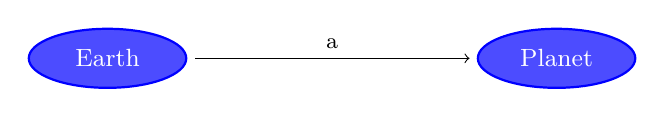
\begin{tikzpicture}[node distance=5cm]
		\node[node style] (Earth) {Earth};
		
		\node[node style, right of=Earth,xshift=2em] (Planet) {Planet}
		   edge [<-] node[edge style=sloped,above]{a} (Earth);
	\end{tikzpicture}
	
	\vspace{2cm}
	
	``Earth is a Planet''
	
\end{frame}

\begin{frame}{RDF}
	
	\begin{itemize}
		\item Knoten und Kanten werden mittels Identifikatoren benannt
		\item Man verwendet dafür \emph{Uniform Resource Identifier} (URI)
		\item Dies unterstützt die (globale) Unterscheidung von Ressourcen
		\item Die URI ist eine Referenz zur beabsichtigen Ressource
		\item Beispiele: Planeten, Bücher, etc. als konzepte oder physische Dinge
	\end{itemize}
	
\end{frame}

\begin{frame}[fragile]{RDF}
	
	\centering
	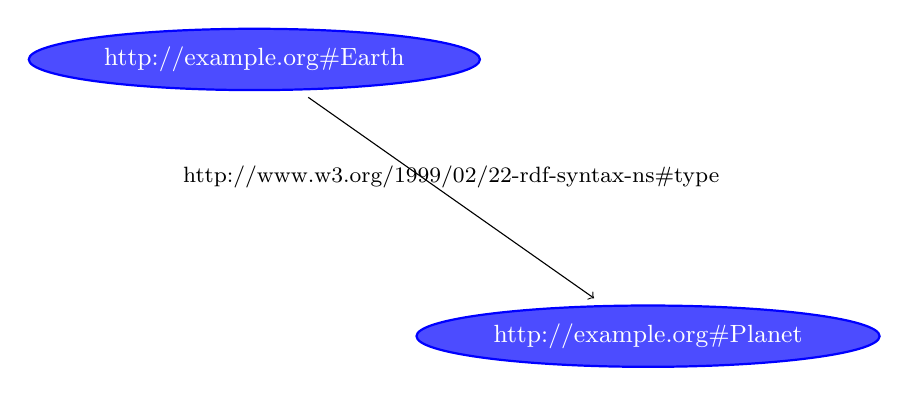
\begin{tikzpicture}[node distance=5cm]
	\node[node style] (Earth) {http://example.org\#Earth};
	
	\node[node style, right of=Earth,yshift=-10em] (Planet) {http://example.org\#Planet}
	   edge [<-] node[edge style,above]{http://www.w3.org/1999/02/22-rdf-syntax-ns\#type} (Earth);
	\end{tikzpicture}
	
\end{frame}

\begin{frame}{URI}
	
	\begin{itemize}
		\item URI ist eine Generalisierung des \emph{Uniform Resource Locator} (URL)
		\item URL ist somit eine Unterart der URI
		\item Jeder URL ist auch ein URI
		\item URL allgemein bekannt als Webadresse, z.B. \texttt{http://google.com}
		\item URL identifiziert \emph{und} lokalisiert eine Ressource
		\item Meist eine digitale Ressource die im Internet lokalisiert ist
		\item Lokalisiert auf einem IP identifizierten Rechner
		\item URI ist ein Identifikator, lediglich identifiziert eine Ressource
		\item Diese Ressource muss nicht digital sein
		\item Zudem muss sie nicht im Internet lokalisiert sein
		\item Tippt man ein URI in den Browser, erhält man u.U. einen Fehler
	\end{itemize}
	
\end{frame}

\begin{frame}{URI}
	
	\begin{itemize}
		\item Im Gegensatz zu URL, gibt es keine Institution die URI vergibt
		\item Eine URL wie z.B. \texttt{markusstocker.com} is registriert
		\item An mehreren Stellen, inklusive Hosting Provider DNS
		\item Man bezahlt für die verschiedenen Services
		\item Ein URI kann man ``einfach so'' erstellen
		\item Wobei es schon ein paar Regeln für ``cool URIs'' gibt
		\item Es ist von Vorteil wenn URIs eindeutig sind
		\item Wobei das nicht gewährleistet wird
		\item Eine Ressource kann durchaus mehrere URIs haben
		\item Zudem kann ein URI für mehrere Ressourcen benutzt werden
		\item URI Aufbau ist wichtig um Änderungsbedarf zu minimieren
		\item Schlecht sind z.B. Technologieabhängigkeiten (wie \texttt{.php}) oder \emph{?query}
	\end{itemize}
	
\end{frame}

\begin{frame}[fragile]{URI Aufbau}
	
	\begin{lstlisting}
	scheme:[//authority]path[?query][#fragment]
	\end{lstlisting}
	
	\vspace{0.5cm}
	
	\begin{itemize}
		\item \texttt{scheme}: Meist \texttt{http}, selbst wenn nicht auf dem Web lokalisiert
		\item Beispiel: \texttt{http://example.org\#Earth} ist ein URI
		\item \texttt{authority}: Meist ein Domänennamen, z.B. \texttt{//example.org}
		\item \texttt{path}: Meist hierarchisch strukturierte Pfade, z.B. \texttt{/astro/vocab}
		\item \texttt{?query}: Optional, für URL Parameter; für URI abgeraten
		\item \texttt{\#fragment}: Wird für URI oft verwendet um Dinge zu identifizieren
	\end{itemize}
	
\end{frame}

\begin{frame}[fragile]{URI Abkürzen}
	
	\begin{itemize}
		\item Es ist möglich URIs abzukürzen
		\item Dies geschieht mittels eines Präfix in Form \texttt{prefix:name}
		\item Der Präfix ist frei wählbar, muss aber definiert werden
		\item Identifikatoren in dieser Form werden auch \emph{qualified names} genannt
		\item Beispiel
		\begin{itemize}
			\item Definiere Präfix \texttt{ex:} für \texttt{http://example.org\#}
			\item Für den URI \texttt{http://example.org\#Earth}
			\item Ergibt sich der ensprechende \emph{qualified name} \texttt{ex:Earth} 
		\end{itemize}
	\end{itemize}
	
\end{frame}

\begin{frame}[fragile]{URI Kürzung in RDF}
	
	\centering
	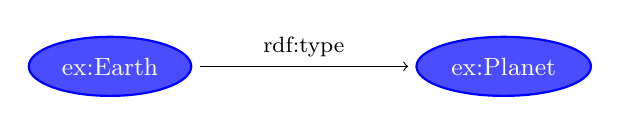
\begin{tikzpicture}[node distance=5cm]
	\node[node style] (Earth) {ex:Earth};
	
	\node[node style, right of=Earth,xshift=0em] (Planet) {ex:Planet}
	edge [<-] node[edge style=sloped,above]{rdf:type} (Earth);
	\end{tikzpicture}
	
\end{frame}

\begin{frame}{RDF Knoten: Nicht nur URI}
	
	\begin{itemize}
		\item In unseren Beispielen waren bisher Knoten mittels URI benannt
		\item In RDF gibt es zwei weitere Knoten Formen
		\item RDF Knoten für Datenwerte, sogenannte \emph{literal} wie z.B. \texttt{6371.0}
		\item Der sogenannte \emph{blank node}, sprich unbenannte Knoten
	\end{itemize}
	
\end{frame}

\begin{frame}{RDF Literal}

	\begin{itemize}
		\item Datenwerte werden in RDF als Literale (\emph{literals}) dargestellt
		\item Der Wert wird generell als Zeichenfolge dargestellt
		\item Zum Beispiel die Folge ``6'' ``3'' ``7'' ``1'' ``.'' ``0''
		\item Die Interpretation der Zeichenfolge wird mittels Datentyp festgelegt
		\item Datentyp ist für Verständnis der beabsichtigten Bedeutung wichtig
		\item Datentyp ist allerdings optional, untypisierte Literale sind möglich
		\item Diese werden immer als Zeichenfolge interpretiert 
		\item Aus einem Literal können keine Kanten ausgehen
		\item Es ist somit nicht möglich Aussagen über Literale zu machen
		\item Literale können auch nicht als Namen für Kanten benutzt werden
	\end{itemize}

\end{frame}

\begin{frame}[fragile]{RDF Literal: Beispiel}
	
	\centering
	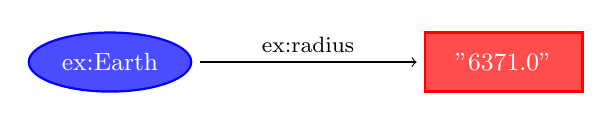
\begin{tikzpicture}[node distance=5cm]
	\node[node style] (Earth) {ex:Earth};
	
	\node[literal style, right of=Earth,xshift=0em] (Radius) {"6371.0"}
	edge [<-] node[edge style=sloped,above]{ex:radius} (Earth);
	\end{tikzpicture}
	
	\vspace{1cm}
	
	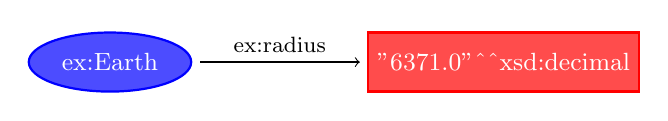
\begin{tikzpicture}[node distance=5cm]
	\node[node style] (Earth) {ex:Earth};
		
	\node[literal style, right of=Earth,xshift=0em] (Radius) {"6371.0"\^{}\^{}xsd:decimal}
	edge [<-] node[edge style=sloped,above]{ex:radius} (Earth);
	\end{tikzpicture}
	
\end{frame}

\begin{frame}[fragile]{RDF Graph}
	
	\centering
	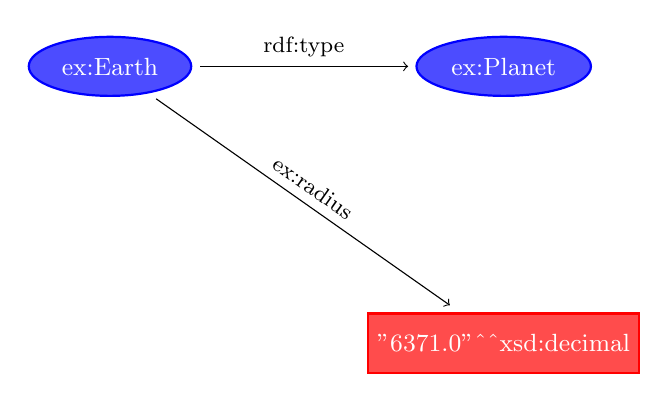
\begin{tikzpicture}[node distance=5cm]
	\node[node style] (Earth) {ex:Earth};
	
	\node[node style, right of=Earth,xshift=0em] (Planet) {ex:Planet}
	edge [<-] node[edge style=sloped,above]{rdf:type} (Earth);
	
	\node[literal style, right of=Earth,yshift=-10em] (Radius) {"6371.0"\^{}\^{}xsd:decimal}
	edge [<-] node[edge style=sloped,above]{ex:radius} (Earth);
	\end{tikzpicture}
	
\end{frame}

\begin{frame}{RDF \emph{Blank Node}}
	
	\begin{itemize}
		\item Unbenannte Knoten die man nicht (global) referenzieren kann
		\item Die Knoten sind nicht mittels URI identifiziert
		\item Keine Ressourcen die man beschreiben möchte
		\item Nur strukturelle Funktion um mehrwertige Relationen darzustellen
		\item Kanten selbst können nicht unbenannt sein
	\end{itemize}
	
\end{frame}

\begin{frame}[fragile]{RDF \emph{Blank Node}: Beispiel}
	
	\centering
	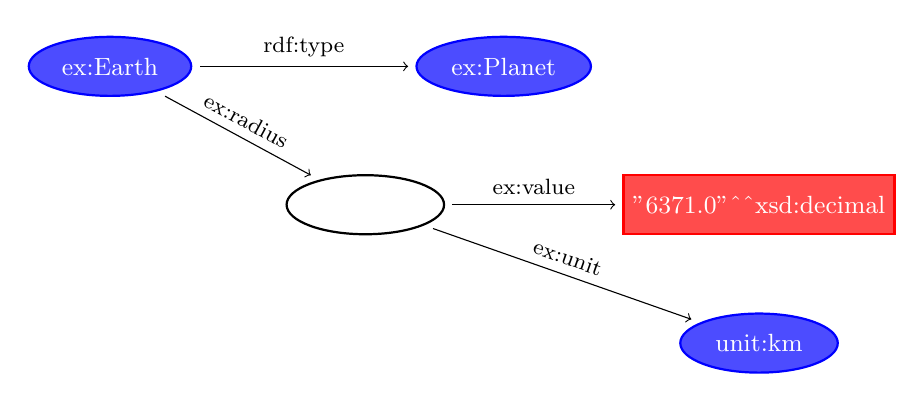
\begin{tikzpicture}[node distance=5cm]
	\node[node style] (Earth) {ex:Earth};
	
	\node[node style, right of=Earth,xshift=0em] (Planet) {ex:Planet}
		edge [<-] node[edge style=sloped,above]{rdf:type} (Earth);
		
	\node[blank style, right of=Earth,xshift=-5em,yshift=-5em] (Radius) {}
	edge [<-] node[edge style=sloped,above]{ex:radius} (Earth);
	
	\node[literal style, right of=Radius,yshift=0em] (RadiusValue) {"6371.0"\^{}\^{}xsd:decimal}
		edge [<-] node[edge style=sloped,above]{ex:value} (Radius);
		
	\node[node style, right of=Radius,yshift=-5em] (RadiusUnit) {unit:km}
			edge [<-] node[edge style=sloped,above]{ex:unit} (Radius);
	\end{tikzpicture}
	
\end{frame}

\begin{frame}{Graphen und Bäume}
	
	\begin{itemize}
		\item XML erzeugt Bäume: Warum RDF Graphen?
		\item Graph Datenstruktur ist wesentlich flexibler
		\item Eine einfache Vereinigung zweiter Graphen ist unproblematisch
		\item Diese dürfen getrennt sein
		\item Die einfache Vereinigung zweiter Bäume ist kein Baum
		\item Man muss weitere Vorkehrungen treffen
		\item Zudem kann man beliebige Knoten einfach relationieren
		\item Bäume haben eine starre Struktur
		\item In Beziehung stehende Information kann im Baum entfernt sein
	\end{itemize}
	
\end{frame}

\begin{frame}{Zusammenfassung}
	
	\begin{itemize}
		\item Sprache zur Beschreibung strukturierter Information
		\item Ist ein grundlegener Baustein des \emph{Semantic Web}
		\item Maschinelle Informationsverarbeitung, Daten und deren Bedeutung
		\item Das \emph{statement} als zentrales RDF Konzept
		\item Eine \emph{statement} Menge (RDF Dokument) spannt einen Graphen
		\item URI als wichtige Technologie zur Benennung von Knoten und Kanten
		\item Graphen sind flexiblere Datenstrukturen als Bäume
	\end{itemize}
	
\end{frame}

\end{document}